\begin{frame}
    \frametitle{Compass}        
    \begin{figure}[!h]        
        \centering
        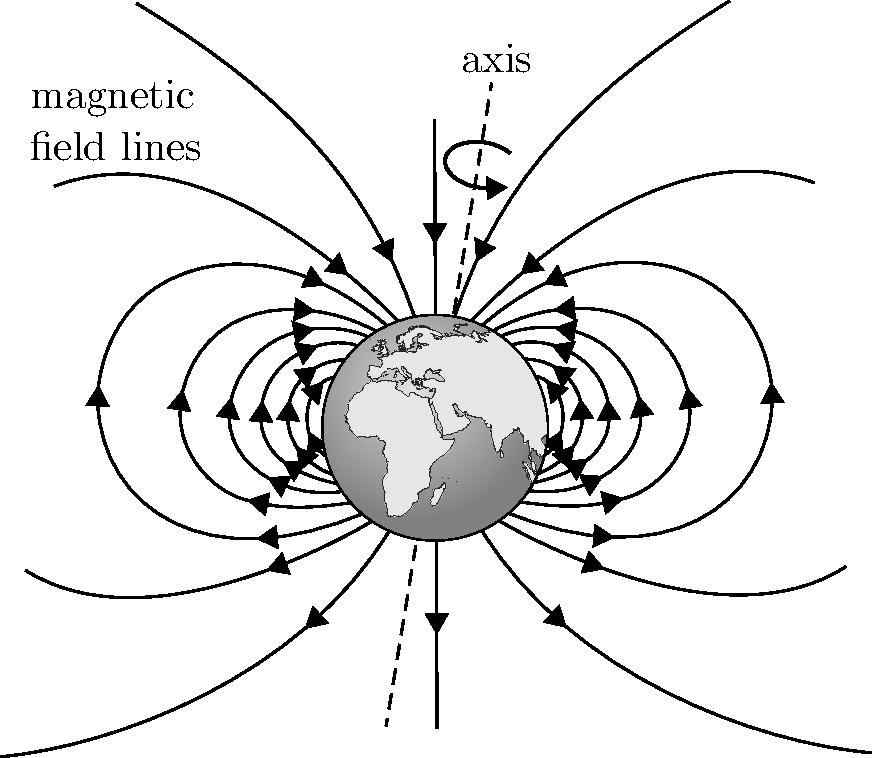
\includegraphics[width=0.3\columnwidth]{images/earth_magnetic_field.pdf}
    \end{figure}
    \footnotesize
    \begin{block}{Principio de funcionamiento}
        La Tierra es un imán masivo pero débil. Los polos de este geomagnético son los polos magnéticos norte y sur de la Tierra, que se mueven constantemente y se encuentran a cierta distancia del eje de rotación del planeta.
        
        En cualquier punto del planeta, las líneas de flujo magnético pueden considerarse un vector $\vec{m}$ cuya magnitud y dirección pueden predecirse y trazarse con precisión. Describimos la dirección del vector en términos de dos ángulos: declinación e inclinación. Una proyección horizontal del vector $\vec{m}$ apunta en la dirección del norte magnético y el ángulo de declinación $D$ se mide desde el norte verdadero, en el sentido de las agujas del reloj hasta esa proyección. El ángulo de inclinación $I$ del vector se mide en un plano vertical hacia abajo desde la horizontal hasta $\vec{m}$. La longitud del vector, la intensidad del campo magnético, se mide con un magnetómetro en unidades de Tesla (T) y para la Tierra varía de $25-\SI{65}{\micro\tesla}$.
    \end{block}
\end{frame}


\begin{frame}
    \frametitle{Compass}
    \footnotesize     
    \begin{figure}[!h]        
        \centering
        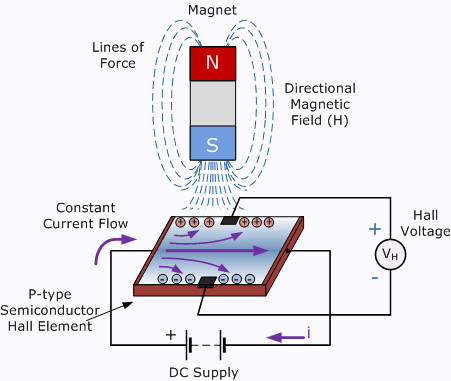
\includegraphics[width=0.3\columnwidth]{electromagnetism.jpg}
    \end{figure}
    
    \begin{block}{Principio de funcionamiento}
        El elemento clave de la mayoría de los magnetómetros modernos es un sensor de efecto Hall, un dispositivo semiconductor que produce un voltaje proporcional a la intensidad del campo magnético en una dirección normal al flujo de corriente. Normalmente, tres sensores de efecto Hall se empaquetan juntos y se disponen de modo que sus ejes sensibles sean ortogonales. Las tres salidas de dicho magnetómetro triaxial son los componentes del vector de intensidad del campo magnético de la Tierra m medido en la estructura del cuerpo $\bodyCoordSystem$.
    \end{block}
\end{frame}

\begin{frame}
    \frametitle{Compass}
    \begin{figure}[!h]        
        \centering
        \subfloat[Magnetic field intensity]
        {
            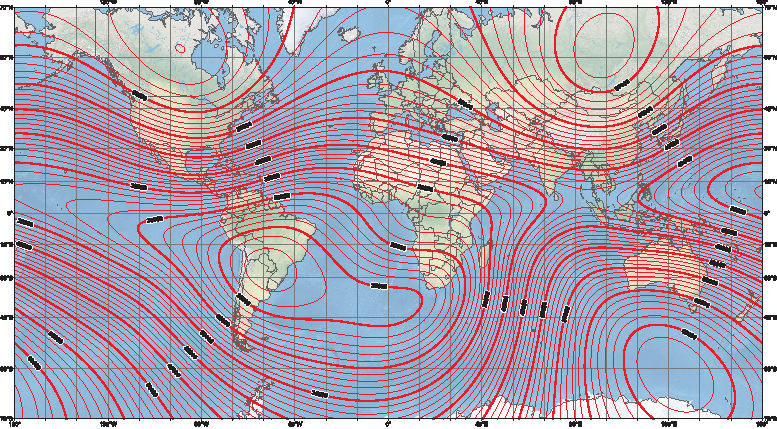
\includegraphics[width=0.5\columnwidth]{images/magnetic_field_intensity.pdf}
        }
        \subfloat[Magnetic declination]
        {
            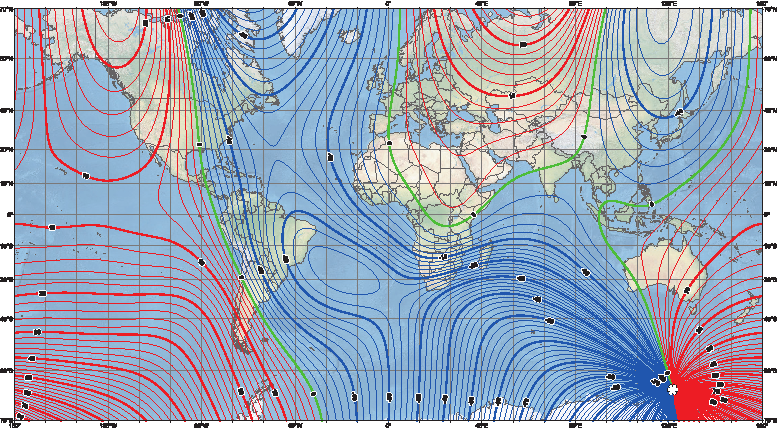
\includegraphics[width=0.5\columnwidth]{images/magnetic_declination.pdf}
        }\\
        \subfloat[Magnetic inclination]
        {
            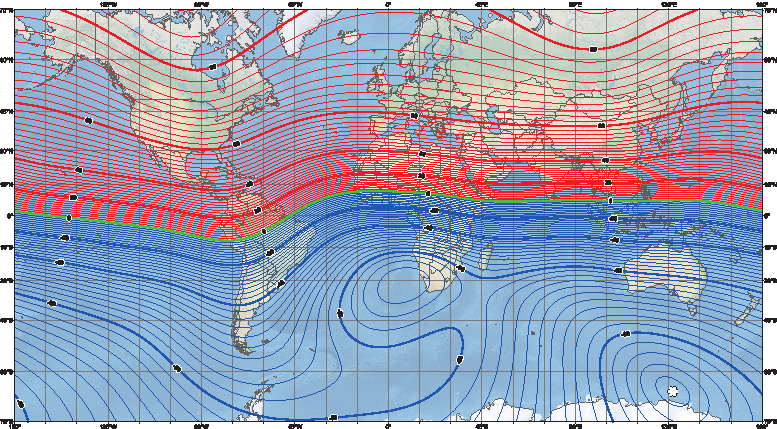
\includegraphics[width=0.5\columnwidth]{images/magnetic_inclination.pdf}
        }
    \end{figure}
\end{frame}


\begin{frame}
    \frametitle{Compass}

    \begin{center}
        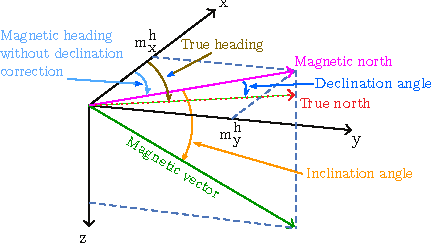
\includegraphics[width=0.5\columnwidth]{images/magnetic_field.pdf}
    \end{center}

    \begin{itemize}
        \item exteroceptivo
        \item
    \end{itemize}
\end{frame}

\begin{frame}
    \frametitle{Compass}

    \begin{center}
        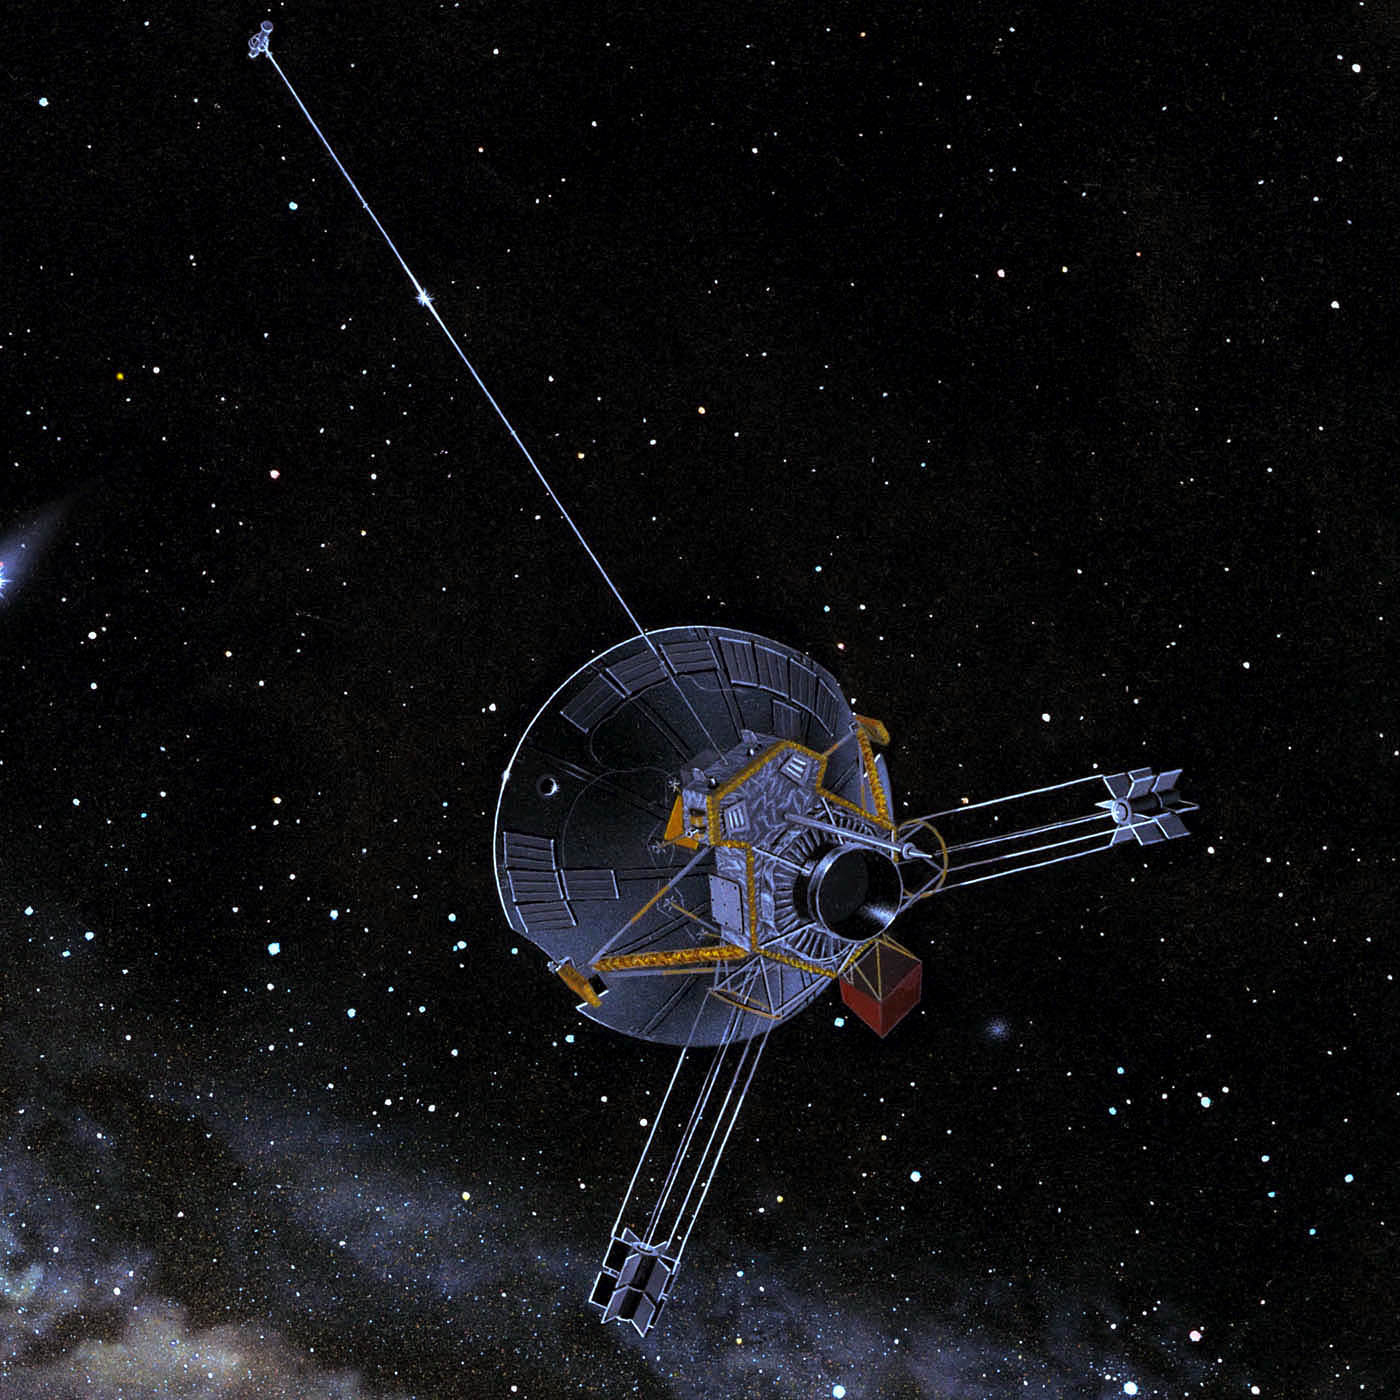
\includegraphics[width=0.5\columnwidth]{pioneer_10.jpg}
    \end{center}
\end{frame}